\subsection*{Диаграмма развертывания приложения}

UML-диаграмма развертывания (deployment diagram) является одной из диаграмм в языке моделирования UML,
которая позволяет визуализировать физическое размещение компонентов программной системы и их взаимосвязи на физических узлах
(например, серверы, компьютеры или устройства).

Диаграмма развертывания позволяет показать, какие компоненты программной системы находятся на каких узлах
и как они взаимодействуют между собой и с внешними ресурсами.
На диаграмме могут быть отображены узлы (физические или виртуальные),
компоненты, связи между ними, а также различные артефакты, такие как файлы или базы данных.

Диаграмма развертывания приложения спроектирована в draw.io и представлена на рис.~\ref{fig:UML_deployment_diagram_prod}.

\begin{figure}[!htb]
    \centering

    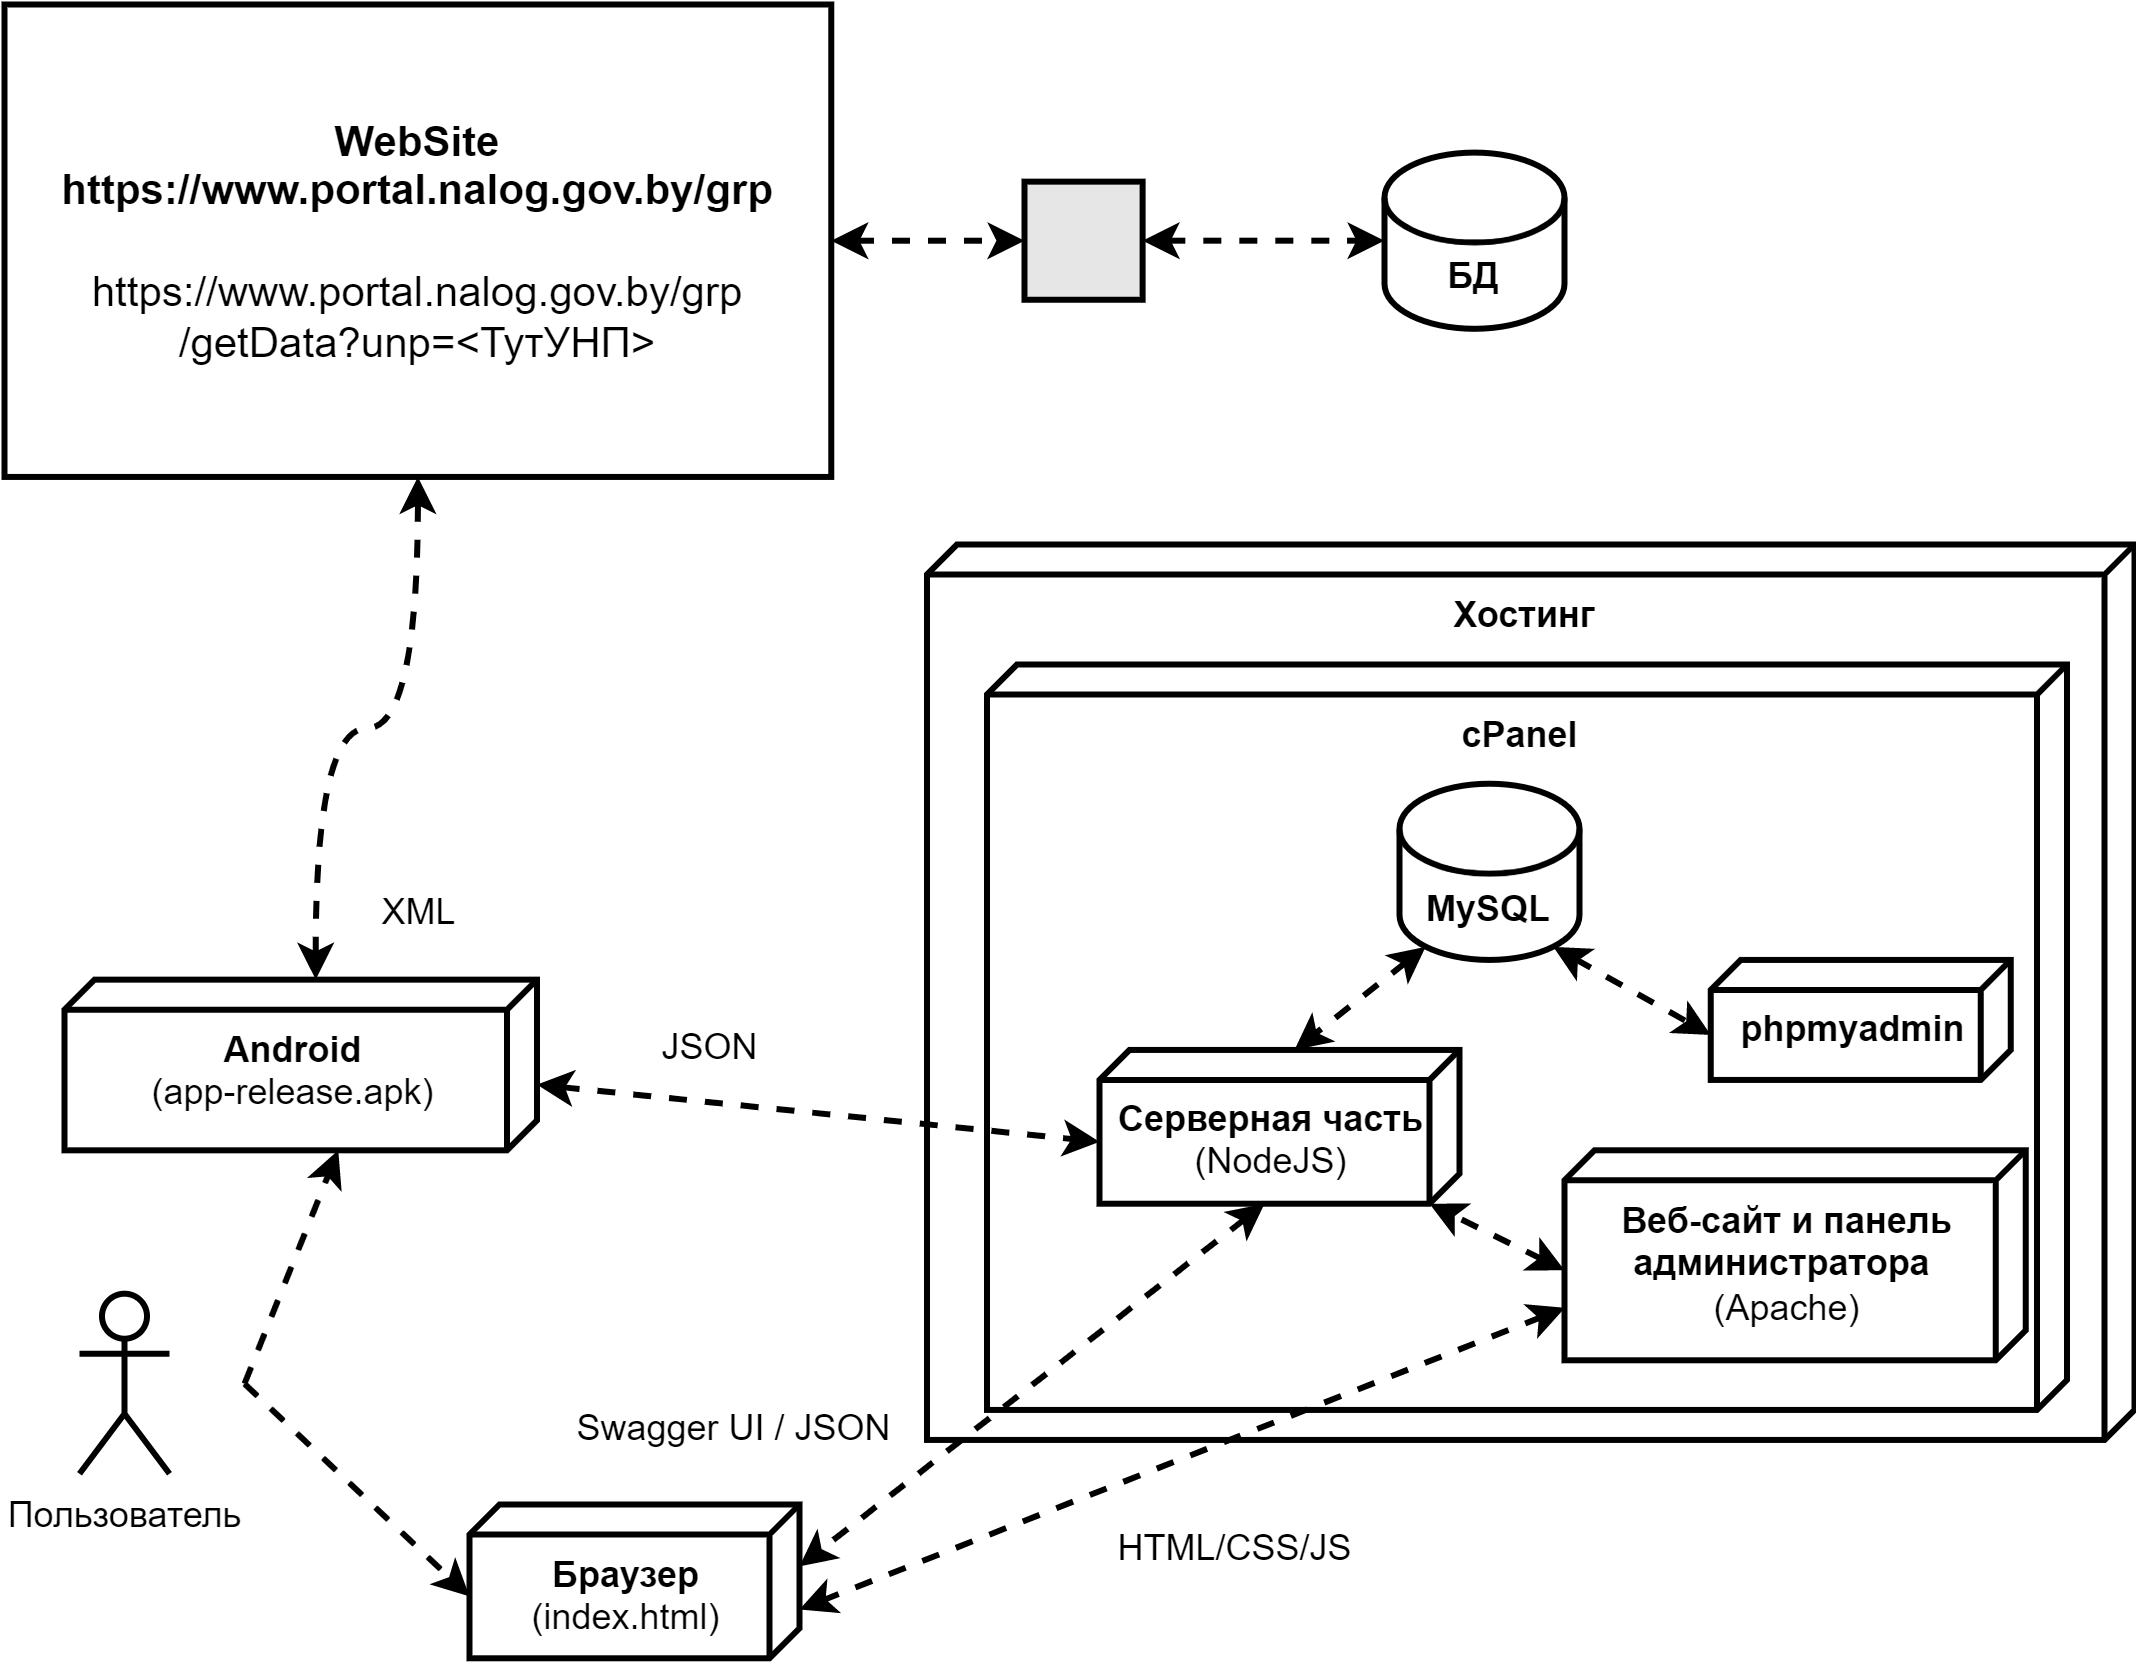
\includegraphics[width=18cm]
    {images/UML/UML_deployment_diagram_prod.png}

    \caption{Диаграмма развертывания приложения}

    \label{fig:UML_deployment_diagram_prod}
\end{figure}
